We can now analyse separately the results for $h_{11}$ and $h_{21}$ for each considered algorithm. We will compare the naive results using the configuration matrix with the most important scalar feature (\texttt{num\_cp}) and the most important vector feature (\texttt{dim\_cp}) and then use the engineered dataset.

\subsection{Linear Regression}
    We first consider the \texttt{LinearRegression} algorithm. We used a \texttt{GridSearchCV} for the hyperparameters \texttt{fit\_intercept} and \texttt{normalize} and we use the \textit{floor} function for the accuracy.
    
    The naive computation with only the matrix components for $h_{11}$ reached $50.6\% \pm 1.1\%$ of accuracy during cross-validation and $50.8\%$ of accuracy for the test predictions using \texttt{fit\_intercept = False} and \texttt{normalize = True}. The same computation for $h_{21}$ led to $10.8\% \pm 1.6\%$ during cross-validation and $12.3\%$ of accuracy in the test set using \texttt{fit\_intercept = True} and \texttt{normalize = False}.
    
    The baseline computation with \texttt{num\_cp} only for $h_{11}$ reached $62\% \pm 2\%$ of accuracy during cross-validation and $63\%$ of accuracy during the test predictions using \texttt{fit\_intercept = True} and \texttt{normalize = True}, thus showing a major improvement in the predictions with respect to the naive case. For $h_{21}$ things get slightly worse in this case with $8.5\% \pm 0.6\%$ of accuracy in cross-validation and $9.2\%$ for the test set using \texttt{fit\_intercept = True} and \texttt{normalize = True}.
    
    The second baseline computation using only \texttt{dim\_cp} shows a worse result for $h_{11}$ with $43.7\% \pm 1.4\%$ in cross-validation and $44.9\%$ of accuracy for the test predictions with \texttt{fit\_intercept = True} and \texttt{normalize = False}, while the results for $h_{21}$ are stable with $8.4\% \pm 0.9\%$ in cross-validation and $8.3\%$ of accuracy for the test set using \texttt{fit\_intercept = False} and \texttt{normalize = True}.
    
    The complete computation using the engineered features improves both $h_{11}$ and $h_{21}$. Specifically we get $52\% \pm 2\%$ of accuracy in cross-validation for $h_{11}$ and $53\%$ during the test predictions using \texttt{fit\_intercept = True} and \texttt{normalize = True}, while the accuracy for $h_{21}$ is almost doubled with $19.4\% \pm 1.6\%$ of accuracy during cross-validation and $20.6\%$ during the test predictions using \texttt{fit\_intercept = False} and \texttt{normalize = True}. We show in Figure~\ref{fig:lin_reg_err} the distribution of the the errors of the test predictions, that is the signed difference between the true value and the prediction.
    
    \begin{figure}[t]
        \centering
        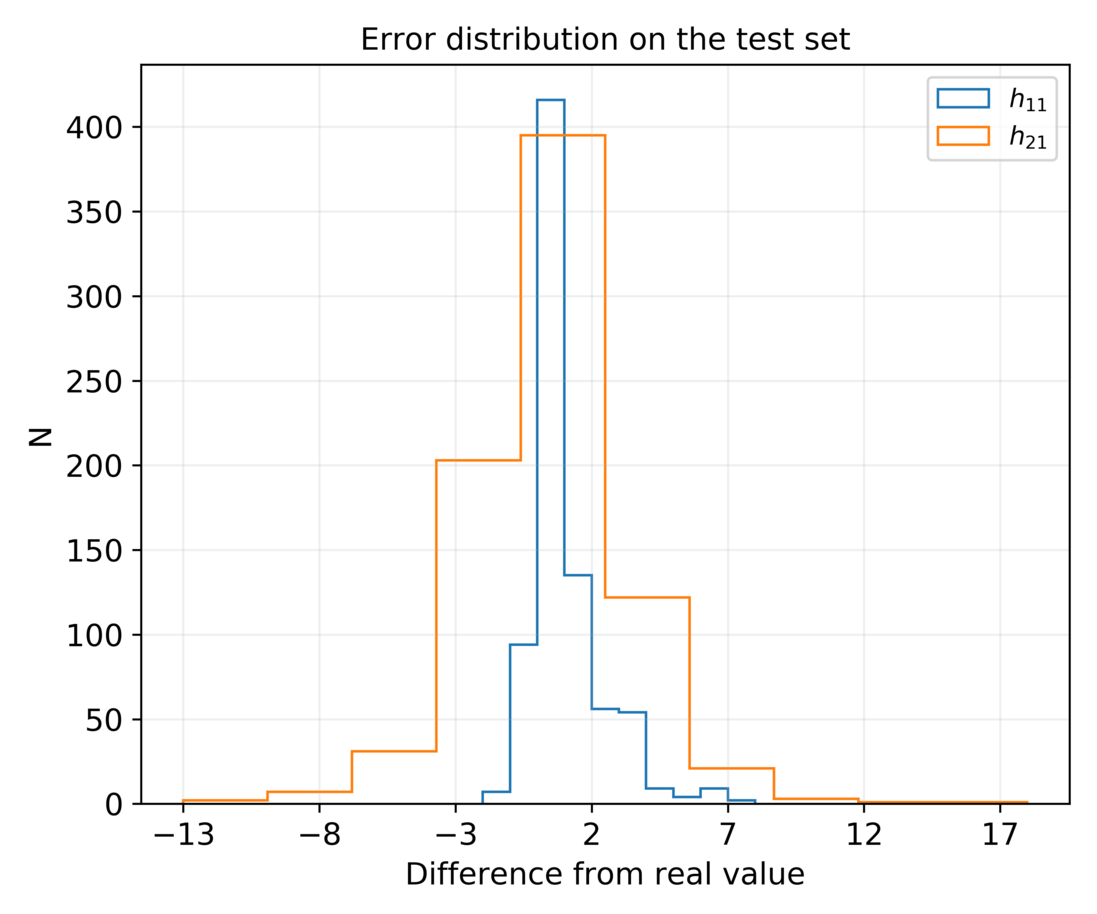
\includegraphics[width=0.75\textwidth]{tex/img/lin_reg_error_eng.png}
        \caption{Error distribution for \texttt{LinearRegression} using the engineered dataset.}
        \label{fig:lin_reg_err}
    \end{figure}
    
\subsection{Lasso Regression}
    We then consider the \texttt{Lasso} algorithm which implements $l1$-regularization with respect to the linear regression algorithm. We implement a search space for the \texttt{BayesSearchCV} for the hyperparameters \texttt{alpha}, \texttt{fit\_intercept}, \texttt{normalize} and \texttt{positive} and we use the \textit{floor} function for the accuracy.
    
    The naive computation with only the matrix components for $h_{11}$ reached $51.0\% \pm 1.5\%$ of accuracy during cross-validation and $50.1\%$ of accuracy for the test predictions using \texttt{alpha = $1.3 \times 10^{-4}$}, \texttt{fit\_intercept = False}, \texttt{normalize = True} and \texttt{positive = True}. The same computation for $h_{21}$ led to $11.4\% \pm 1.2\%$ during cross-validation and $13.0\%$ of accuracy in the test set using \texttt{alpha = $1.4 \times 10^{-4}$}, \texttt{fit\_intercept = True}, \texttt{normalize = True} and \texttt{positive = False}.
    
    The baseline computation with \texttt{num\_cp} only for $h_{11}$ reached $62\% \pm 2\%$ of accuracy during cross-validation and $63\%$ of accuracy during the test predictions using \texttt{alpha = $4.0$}, \texttt{fit\_intercept = False}, \texttt{normalize = True} and \texttt{positive = True}, thus showing a major improvement in the predictions with respect to the naive case. For $h_{21}$ we find $12.0\% \pm 0.7\%$ of accuracy in cross-validation and $12.3\%$ for the test set using \texttt{alpha = $2.4$}, \texttt{fit\_intercept = True}, \texttt{normalize = False} and \texttt{positive = False}.
    
    The second baseline computation using only \texttt{dim\_cp} shows a worse result for $h_{11}$ with $43.7\% \pm 1.5\%$ in cross-validation and $44.9\%$ of accuracy for the test predictions with \texttt{alpha = $8.0 \times 10^{-4}$}, \texttt{fit\_intercept = True}, \texttt{normalize = False} and \texttt{positive = False}, while the results for $h_{21}$ are $8.5\% \pm 0.9\%$ in cross-validation and $8.7\%$ of accuracy for the test set using \texttt{alpha = $1.6 \times 10^{-2}$}, \texttt{fit\_intercept = False}, \texttt{normalize = False} and \texttt{positive = False}.
    
    The complete computation using the engineered features improves both $h_{11}$ and $h_{21}$. Specifically we get $63\% \pm 2\%$ of accuracy in cross-validation for $h_{11}$ and $64\%$ during the test predictions using \texttt{alpha = $8.0 \times 10^{-2}$}, \texttt{fit\_intercept = False}, \texttt{normalize = False} and \texttt{positive = False}, while the accuracy for $h_{21}$ is almost doubled with $20\% \pm 2\%$ of accuracy during cross-validation and $18\%$ during the test predictions using \texttt{alpha = $2.3 \times 10^{-3}$}, \texttt{fit\_intercept = False}, \texttt{normalize = True} and \texttt{positive = False}. We show in Figure~\ref{fig:lasso_err} the distribution of the the errors of the test predictions.
    
    \begin{figure}[t]
        \centering
        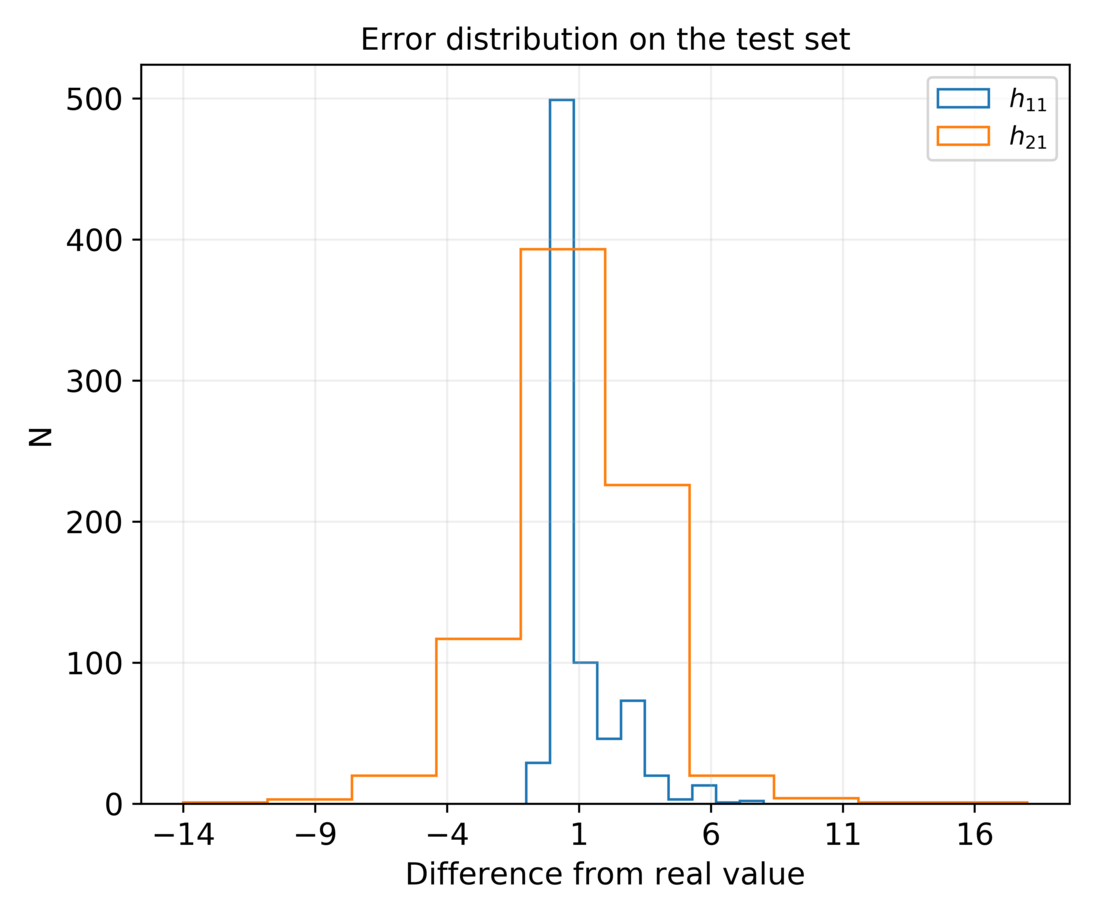
\includegraphics[width=0.75\textwidth]{tex/img/lasso_error_eng.png}
        \caption{Error distribution for \texttt{Lasso} using the engineered dataset.}
        \label{fig:lasso_err}
    \end{figure}
    
\subsection{Ridge Regression}
    We then consider the \texttt{Ridge} algorithm which implements $l2$ regularisation of the fit parameters. We implement a search space for the \texttt{BayesSearchCV} for the hyperparameters \texttt{alpha}, \texttt{fit\_intercept}, \texttt{normalize} and we use the \textit{floor} function for the accuracy.
    
    The naive computation with only the matrix components for $h_{11}$ reached $50.9\% \pm 1.1\%$ of accuracy during cross-validation and $50.0\%$ of accuracy for the test predictions using \texttt{alpha = $3.2$}, \texttt{fit\_intercept = False} and \texttt{normalize = True}. The same computation for $h_{21}$ led to $11.4\% \pm 1.0\%$ during cross-validation and $12.2\%$ of accuracy in the test set using \texttt{alpha = $9.1 \times 10^{-3}$}, \texttt{fit\_intercept = True} and \texttt{normalize = True}.
    
    The baseline computation with \texttt{num\_cp} only for $h_{11}$ reached $62\% \pm 2\%$ of accuracy during cross-validation and $63\%$ of accuracy during the test predictions using \texttt{alpha = $1.4 \times 10^{-2}$}, \texttt{fit\_intercept = True} and \texttt{normalize = True}, thus showing a major improvement in the predictions with respect to the naive case. For $h_{21}$ we find $12.0\% \pm 0.7\%$ of accuracy in cross-validation and $12.3\%$ for the test set using \texttt{alpha = $0.29$}, \texttt{fit\_intercept = True} and \texttt{normalize = True}.
    
    The second baseline computation using only \texttt{dim\_cp} shows a worse result for $h_{11}$ with $45.2\% \pm 1.6\%$ in cross-validation and $46.3\%$ of accuracy for the test predictions with \texttt{alpha = $0.11$}, \texttt{fit\_intercept = True} and \texttt{normalize = True}, while the results for $h_{21}$ are $8.7\% \pm 1.0\%$ in cross-validation and $9.7\%$ of accuracy for the test set using \texttt{alpha = $0.34$}, \texttt{fit\_intercept = True} and \texttt{normalize = True}.
    
    The complete computation using the engineered features does not improve $h_{11}$ but the results for $h_{21}$ get better. Specifically we get $55\% \pm 3\%$ of accuracy in cross-validation for $h_{11}$ and $55\%$ during the test predictions using \texttt{alpha = $100.0$}, \texttt{fit\_intercept = True} and \texttt{normalize = False}, while the accuracy for $h_{21}$ is almost doubled with $19.6\% \pm 1.6\%$ of accuracy during cross-validation and $20.1\%$ during the test predictions using \texttt{alpha = $0.18$}, \texttt{fit\_intercept = False} and \texttt{normalize = False}. We show in Figure~\ref{fig:ridge_err} the distribution of the the errors of the test predictions.
    
    \begin{figure}[t]
        \centering
        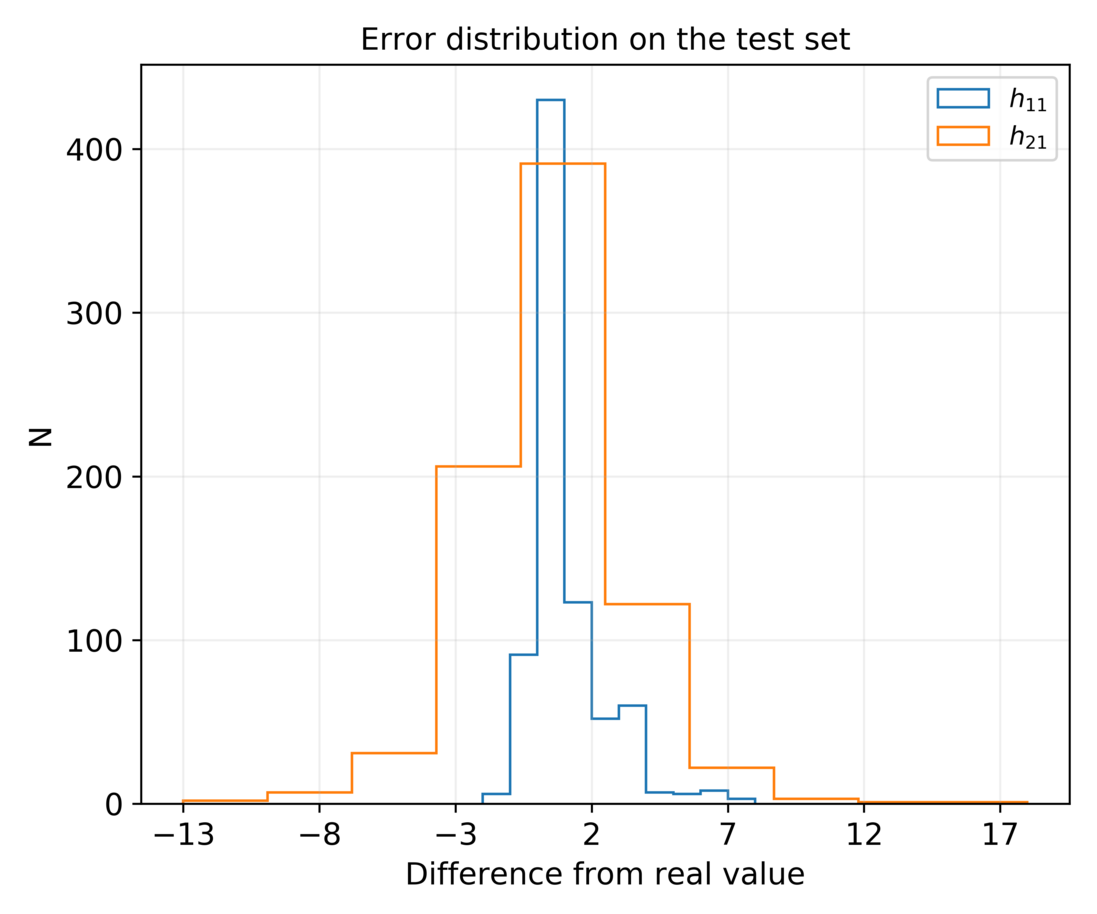
\includegraphics[width=0.75\textwidth]{tex/img/ridge_error_eng.png}
        \caption{Error distribution for \texttt{Ridge} using the engineered dataset.}
        \label{fig:ridge_err}
    \end{figure}
    
\subsection{Elastic Net Regression}
    We then consider the \texttt{ElasticNet} algorithm which implements both $l1$ and $l2$ regularisation. We implement a search space for the \texttt{BayesSearchCV} for the hyperparameters \texttt{alpha}, \texttt{fit\_intercept}, \texttt{l1\_ratio}, \texttt{normalize} and \texttt{positive} and we use the \textit{floor} function for the accuracy.
    
    The naive computation with only the matrix components for $h_{11}$ reached $51.5\% \pm 1.6\%$ of accuracy during cross-validation and $51.1\%$ of accuracy for the test predictions using \texttt{alpha = $2.9 \times 10^{-6}$}, \texttt{fit\_intercept = True}, \texttt{l1\_ratio = 0.0}, \texttt{normalize = True} and \texttt{positive = True}. The same computation for $h_{21}$ led to $11.4\% \pm 1.3\%$ during cross-validation and $9.9\%$ of accuracy in the test set using \texttt{alpha = $3.6 \times 10^{-4}$}, \texttt{fit\_intercept = True}, \texttt{l1\_ratio = $1.0$}, \texttt{normalize = True} and \texttt{positive = False}.
    
    The baseline computation with \texttt{num\_cp} only for $h_{11}$ reached $62\% \pm 2\%$ of accuracy during cross-validation and $63\%$ of accuracy during the test predictions using \texttt{alpha = $3.2 \times 10^{-2}$}, \texttt{fit\_intercept = True}, \texttt{l1\_ratio = $0.18$}, \texttt{normalize = False} and \texttt{positive = False}, thus showing a major improvement in the predictions with respect to the naive case. For $h_{21}$ we find $12.0\% \pm 0.7\%$ of accuracy in cross-validation and $12.3\%$ for the test set using \texttt{alpha = $2.8$}, \texttt{fit\_intercept = True}, \texttt{l1\_ratio = $1.0$}, \texttt{normalize = False} and \texttt{positive = False}.
    
    The second baseline computation using only \texttt{dim\_cp} shows a worse result for $h_{11}$ with $45\% \pm 2\%$ in cross-validation and $46\%$ of accuracy for the test predictions with \texttt{alpha = $1.3 \times 10^{-5}$}, \texttt{fit\_intercept = True}, \texttt{l1\_ratio = 0.0}, \texttt{normalize = True} and \texttt{positive = True}, while the results for $h_{21}$ are $9.6\% \pm 0.7\%$ in cross-validation and $9.5\%$ of accuracy for the test set using \texttt{alpha = $0.16$}, \texttt{fit\_intercept = False}, \texttt{l1\_ratio = 0.0}, \texttt{normalize = False} and \texttt{positive = False}.
    
    The complete computation using the engineered features improves both $h_{11}$ and $h_{21}$. Specifically we get $62\% \pm 2\%$ of accuracy in cross-validation for $h_{11}$ and $63\%$ during the test predictions using \texttt{alpha = $0.6$}, \texttt{fit\_intercept = False}, \texttt{l1\_ratio = 0.0}, \texttt{normalize = False} and \texttt{positive = False}, while the accuracy for $h_{21}$ is almost doubled with $19.9\% \pm 1.4\%$ of accuracy during cross-validation and $18.3\%$ during the test predictions using \texttt{alpha = $1.1 \times 10^{-3}$}, \texttt{fit\_intercept = False}, \texttt{l1\_ratio = $0.0$}, \texttt{normalize = True} and \texttt{positive = False}. We show in Figure~\ref{fig:el_net_err} the distribution of the the errors of the test predictions.
    
    Notice that in almost all cases the penalty was entirely $l1$ or $l2$: there is no mixing of the regularisations. Given the direct results of \texttt{Lasso} and \textit{Ridge} we are however confident that the best regularisation is $l1$: it directly gives the best accuracy results on the predictions.
    
    \begin{figure}[t]
        \centering
        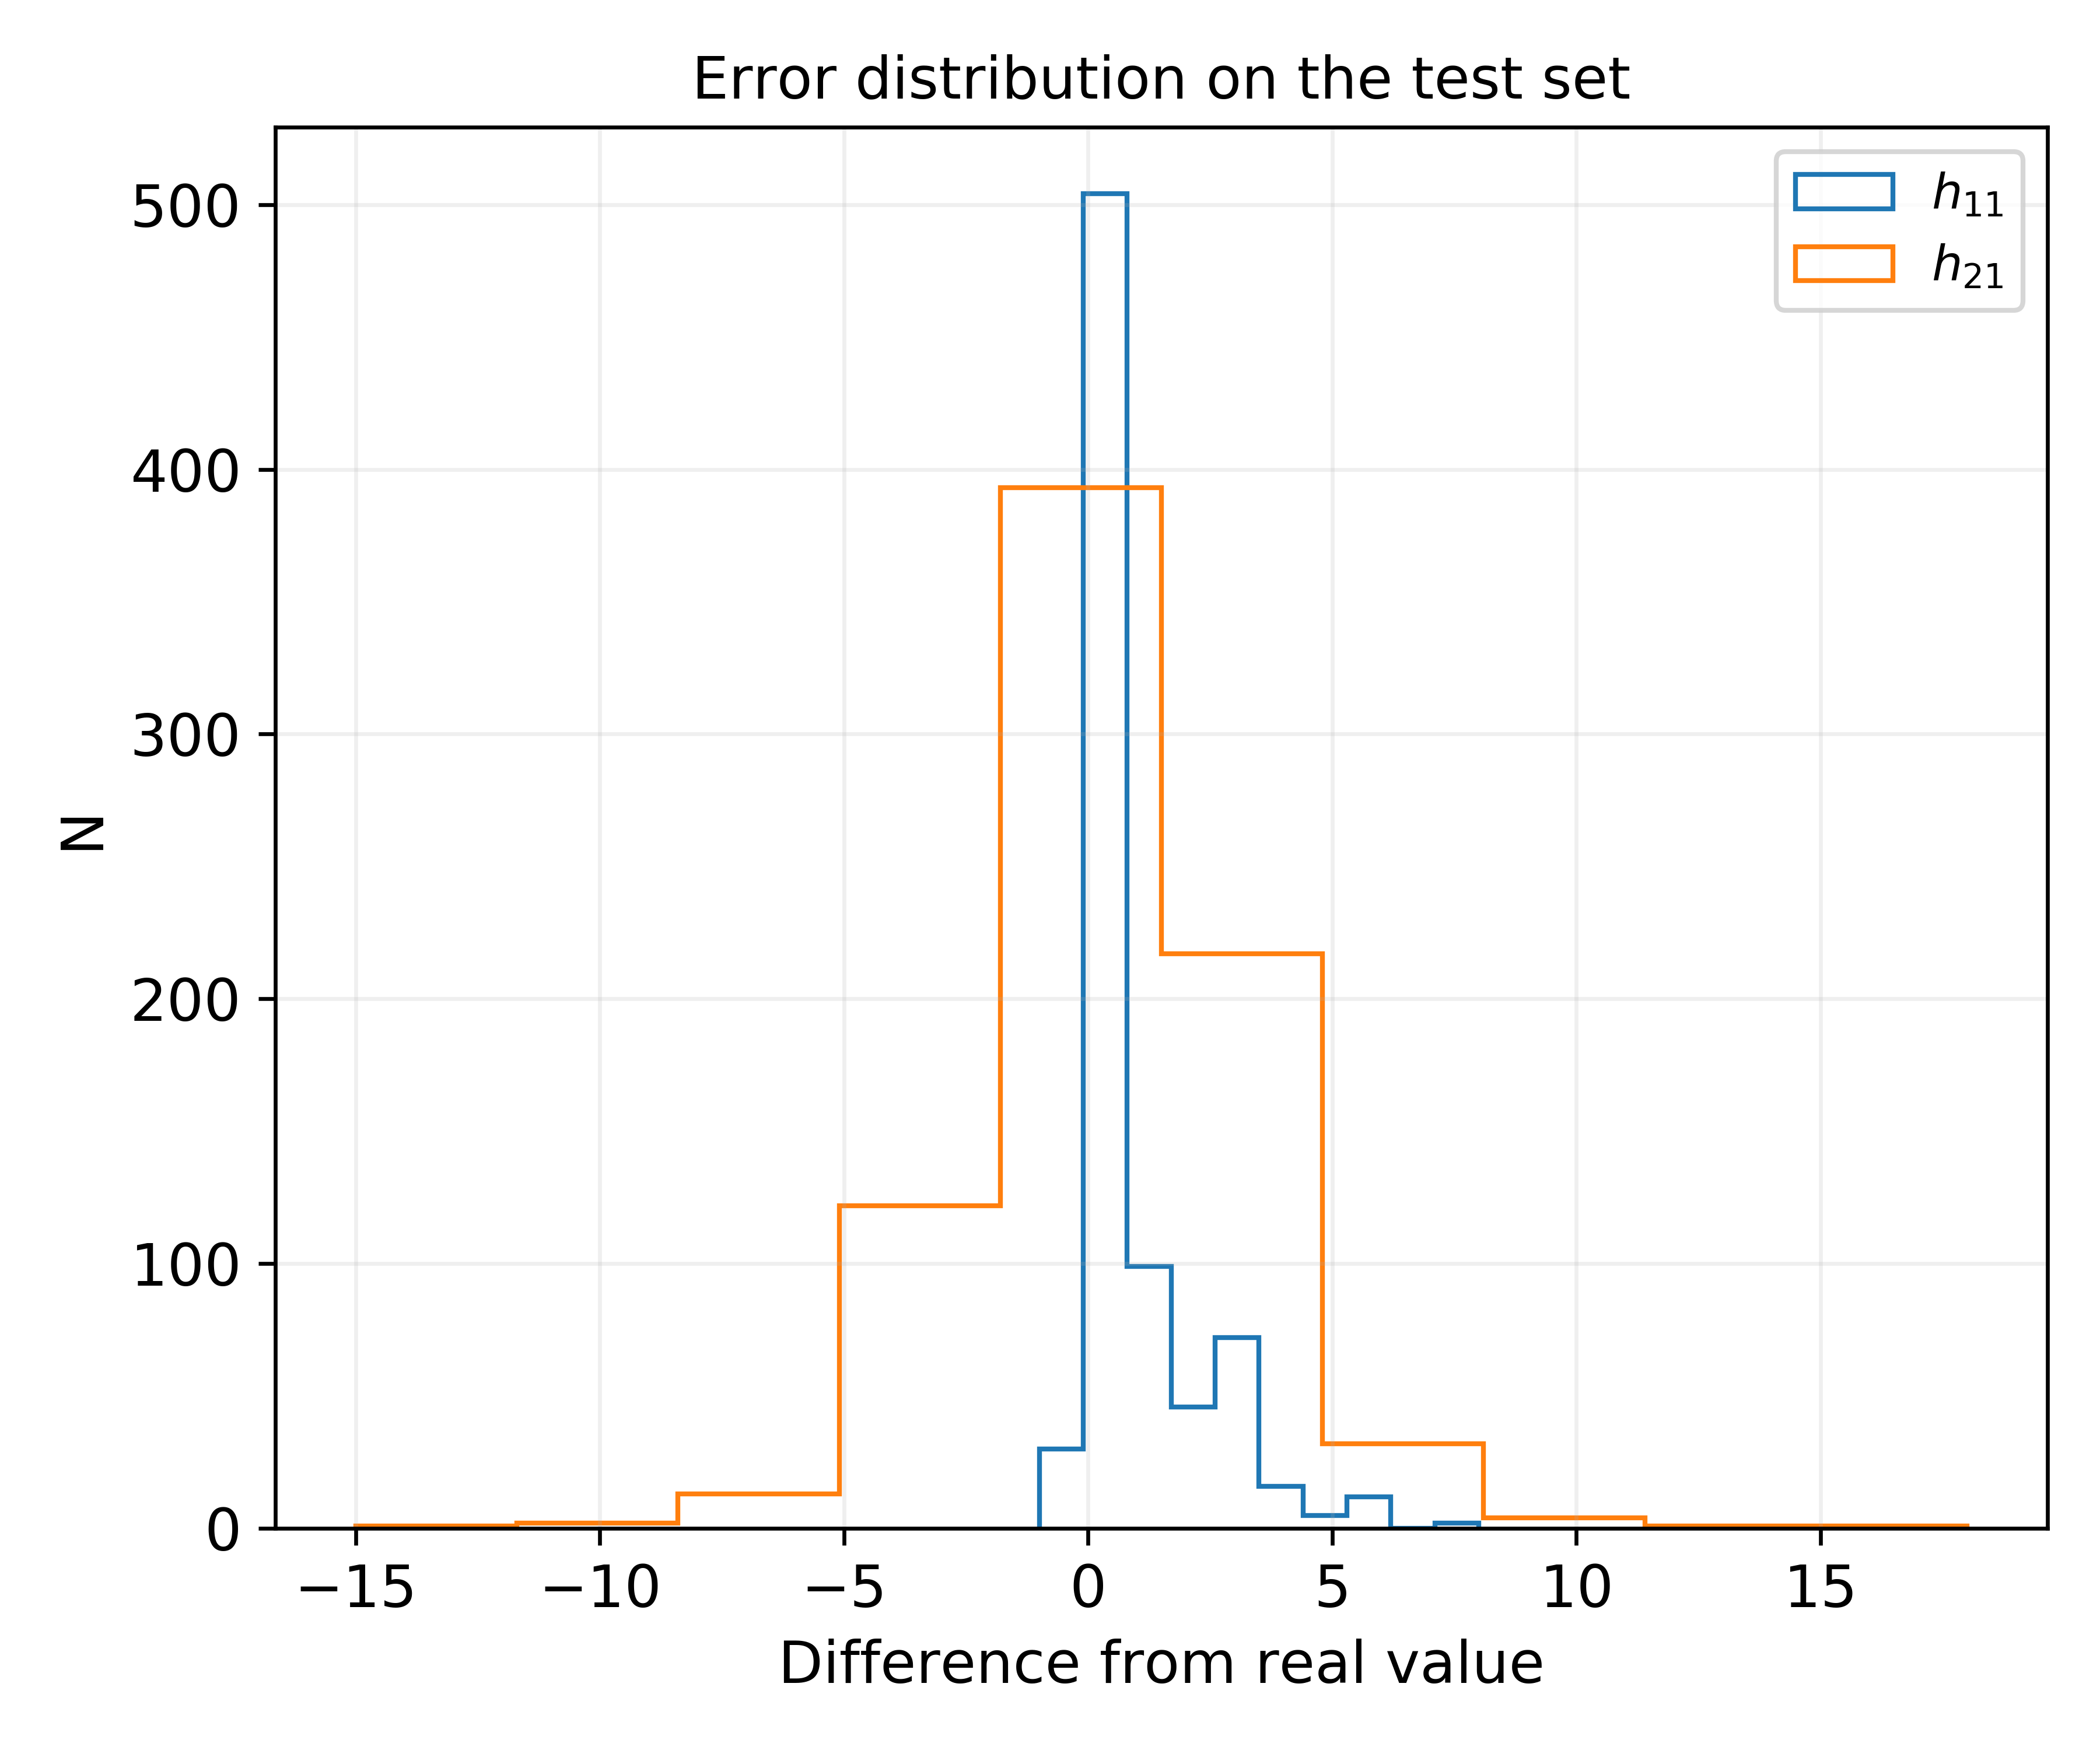
\includegraphics[width=0.75\textwidth]{tex/img/el_net_error_eng.png}
        \caption{Error distribution for \texttt{ElasticNet} using the engineered dataset.}
        \label{fig:el_net_err}
    \end{figure}
    
\subsection{Linear Support Vector}
    We then consider the \texttt{LinearSVR} algorithm. We implement a search space for the \texttt{BayesSearchCV} for the hyperparameters \texttt{C}, \texttt{fit\_intercept}, \texttt{intercept\_scaling} and \texttt{loss} and we use the \textit{floor} function for the accuracy.
    
    The naive computation with only the matrix components for $h_{11}$ reached $50.9\% \pm 1.1\%$ of accuracy during cross-validation and $50.1\%$ of accuracy for the test predictions using  \texttt{C = $0.15$}, \texttt{fit\_intercept = False}, \texttt{intercept\_scaling = $100.0$} and \texttt{loss = squared\_epsilon\_insensitive}. The same computation for $h_{21}$ led to $11.5\% \pm 1.0\%$ during cross-validation and $8.0\%$ of accuracy in the test set using \texttt{C = $0.5$}, \texttt{fit\_intercept = True}, \texttt{intercept\_scaling = $0.96$} and \texttt{loss = epsilon\_insensitive}.
    
    The baseline computation with \texttt{num\_cp} only for $h_{11}$ reached $62\% \pm 2\%$ of accuracy during cross-validation and $0\%$ of accuracy\footnote{As of March, 16th I am still looking for the bug. However the results shown later do not present such issue.} during the test predictions using \texttt{C = $0.01$}, \texttt{fit\_intercept = False}, \texttt{intercept\_scaling = $0.015$} and \texttt{loss = epsilon\_insensitive}, thus showing a major improvement in the predictions with respect to the naive case. For $h_{21}$ we find $12.0\% \pm 0.7\%$ of accuracy in cross-validation and $12.3\%$ for the test set using \texttt{C = $1 \times 10^{-4}$}, \texttt{fit\_intercept = True}, \texttt{intercept\_scaling = $100.0$} and \texttt{loss = squared\_epsilon\_insensitive}.
    
    The second baseline computation using only \texttt{dim\_cp} shows a worse result for $h_{11}$ with $48\% \pm 2\%$ in cross-validation and $46\%$ of accuracy for the test predictions with \texttt{C = $7.4 \times 10^{-3}$}, \texttt{fit\_intercept = True}, \texttt{intercept\_scaling = $46.7$} and \texttt{loss = epsilon\_insensitive}, while the results for $h_{21}$ are $9.6\% \pm 0.5\%$ in cross-validation and $9.4\%$ of accuracy for the test set using \texttt{C = $6.7 \times 10^{-4}$}, \texttt{fit\_intercept = True}, \texttt{intercept\_scaling = $0.01$} and \texttt{loss = squared\_epsilon\_insensitive}.
    
    The complete computation using the engineered features improves both $h_{11}$ and $h_{21}$. Specifically we get $62\% \pm 2\%$ of accuracy in cross-validation for $h_{11}$ and $64\%$ during the test predictions using \texttt{C = $1.4 \times 10^{-4}$}, \texttt{fit\_intercept = False}, \texttt{intercept\_scaling = $0.02$} and \texttt{loss = squared\_epsilon\_insensitive}, while the accuracy for $h_{21}$ is almost doubled with $21\% \pm 2\%$ of accuracy during cross-validation and $20\%$ during the test predictions using \texttt{C = $1.4$}, \texttt{fit\_intercept = False}, \texttt{intercept\_scaling = $0.01$} and \texttt{loss = epsilon\_insensitive}. We show in Figure~\ref{fig:lin_svr_err} the distribution of the the errors of the test predictions.
    
    \begin{figure}[t]
        \centering
        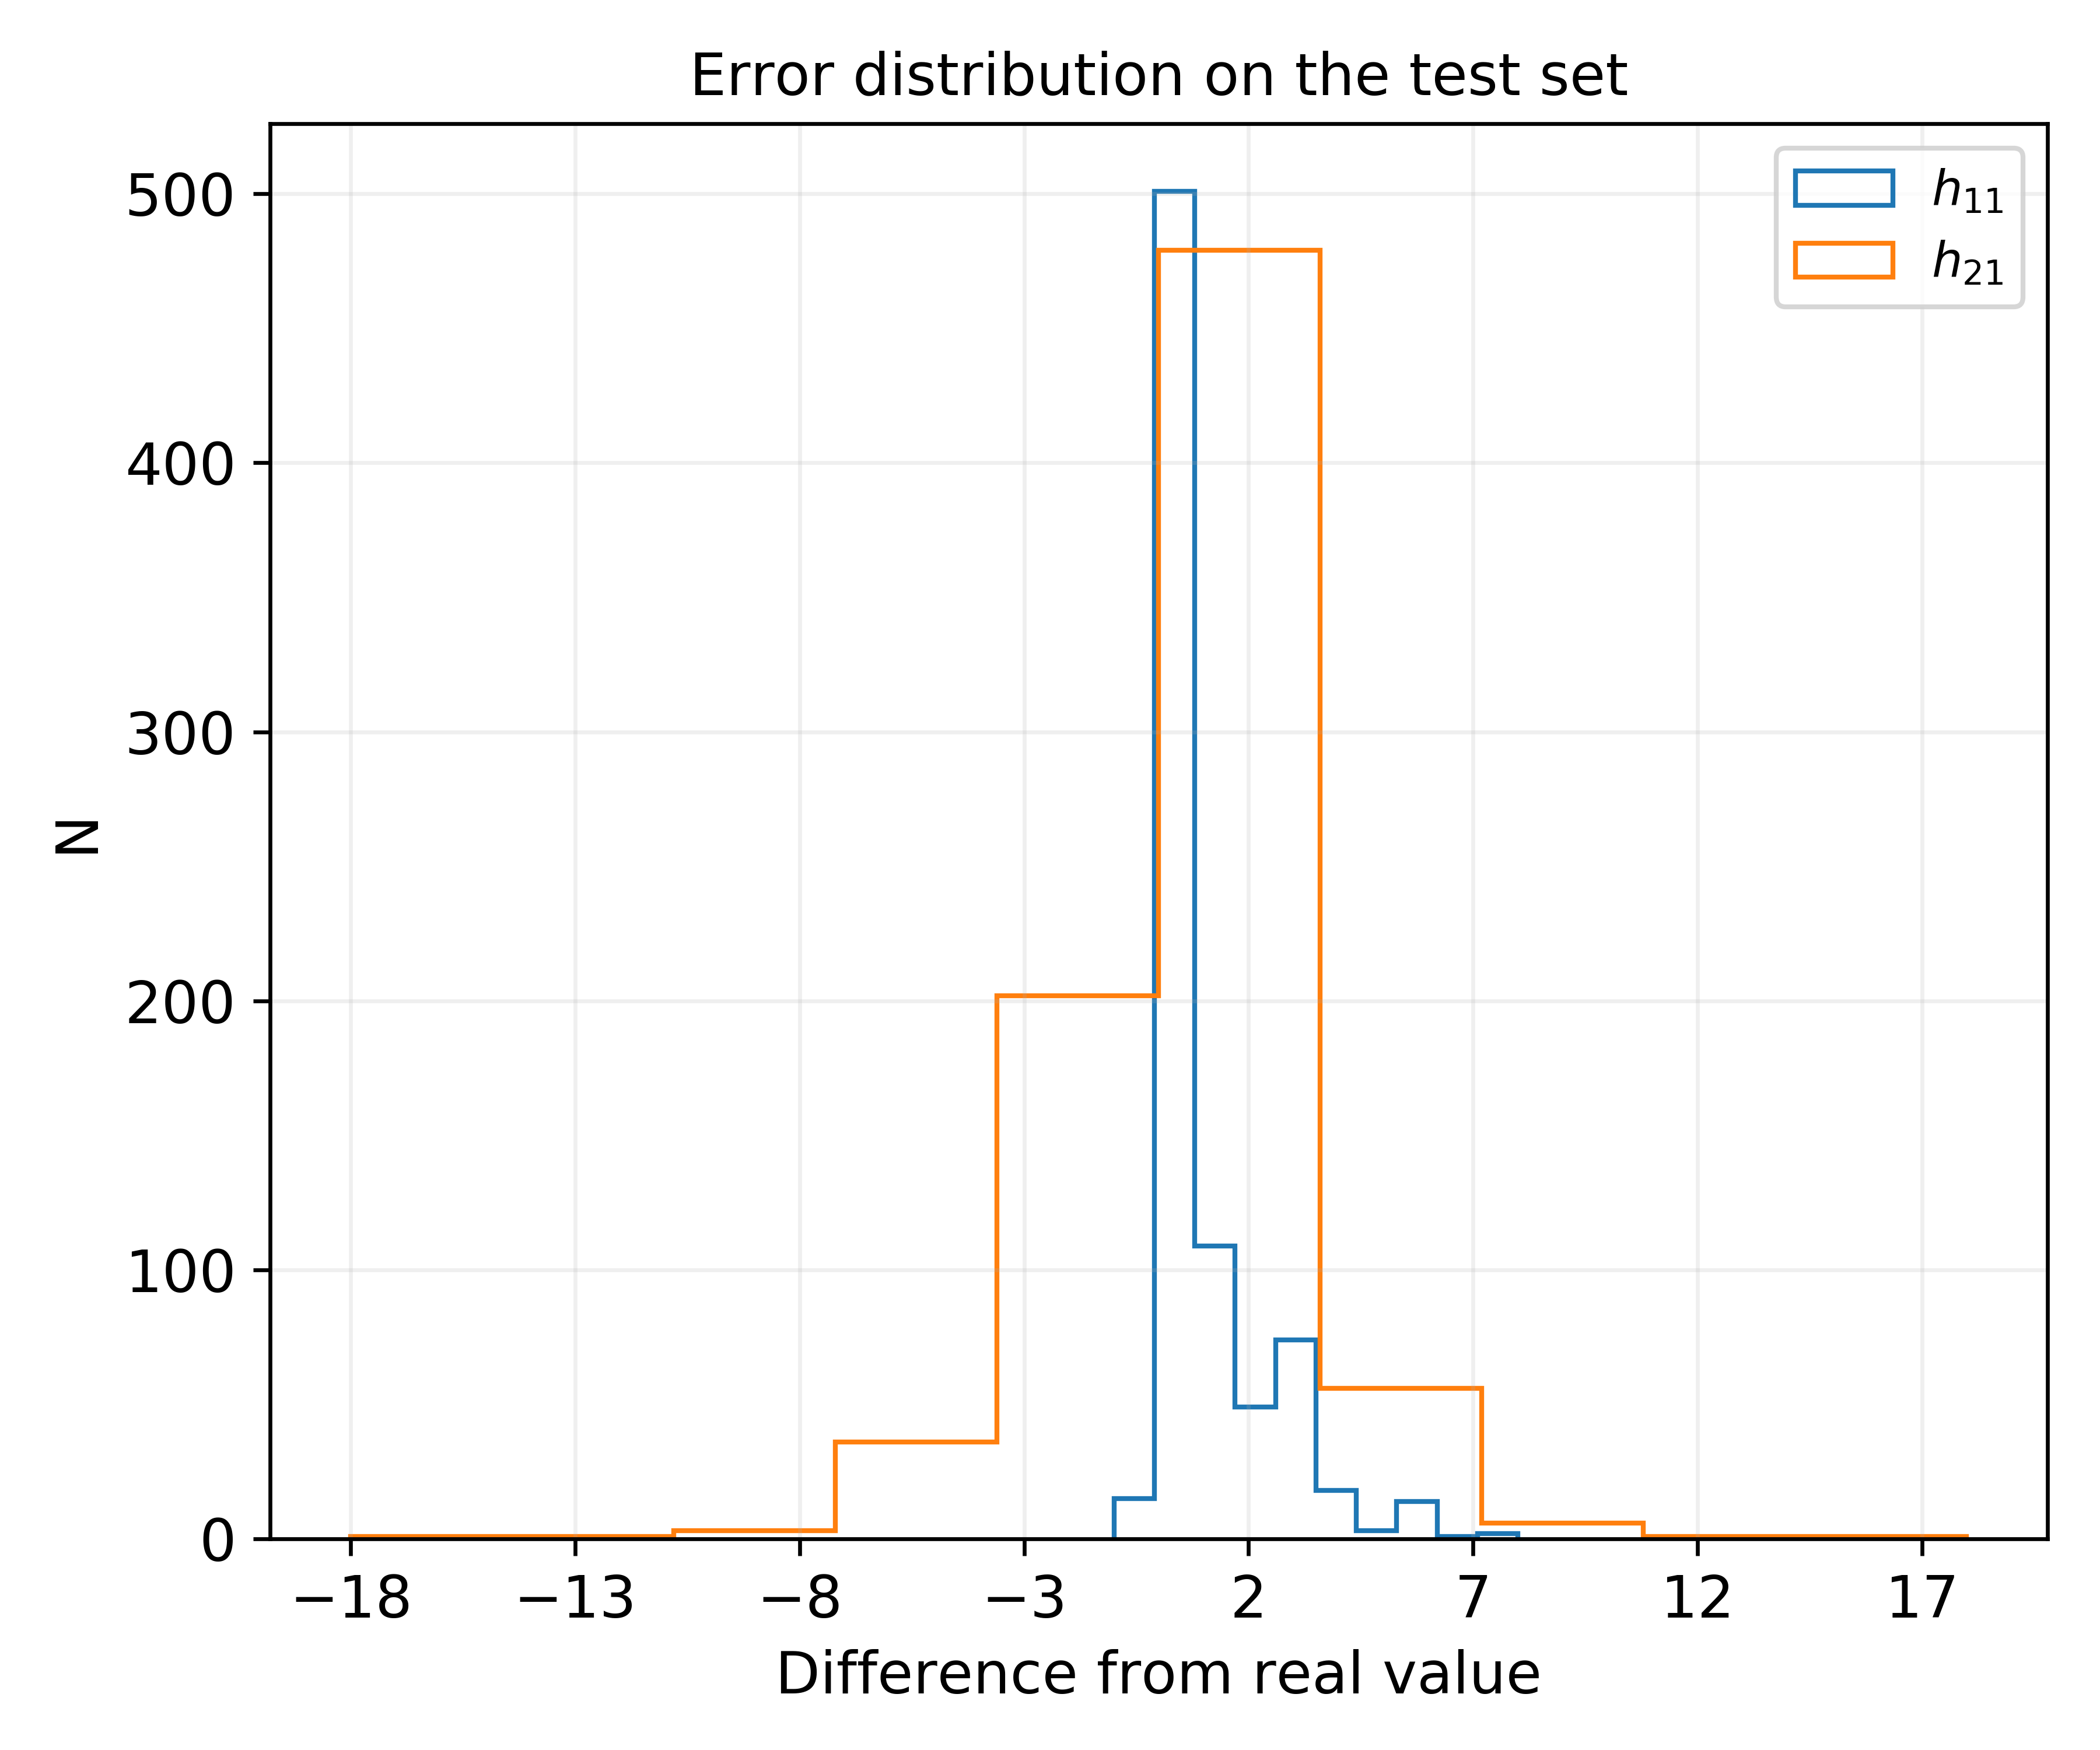
\includegraphics[width=0.75\textwidth]{tex/img/lin_svr_error_eng.png}
        \caption{Error distribution for \texttt{LinearSVR} using the engineered dataset.}
        \label{fig:lin_svr_err}
    \end{figure}
    
\subsection{Gaussian Support Vector}
    We then consider the \texttt{SVR} algorithm with \textit{rbf} kernel. We implement a search space for the \texttt{BayesSearchCV} for the hyperparameters \texttt{C}, \texttt{epsilon}, \texttt{gamma} and \texttt{shrinking} and we use the \textit{rint} function for the accuracy.
    
    The naive computation with only the matrix components for $h_{11}$ reached $69.6\% \pm 1.6\%$ of accuracy during cross-validation and $70.4\%$ of accuracy for the test predictions using \texttt{C = $9.94$}, \texttt{epsilon = $3.1 \times 10^{-5}$}, \texttt{gamma = $0.06$} and \texttt{shrinking = True}. The same computation for $h_{21}$ led to $22.3\% \pm 1.2\%$ during cross-validation and $21.5\%$ of accuracy in the test set using \texttt{C = $34.1$}, \texttt{epsilon = $1.0 \times 10^{-5}$}, \texttt{gamma = $0.04$} and \texttt{shrinking = False}.
    
    The baseline computation with \texttt{num\_cp} only for $h_{11}$ reached $62\% \pm 2\%$ of accuracy during cross-validation and $63\%$ of accuracy during the test predictions using \texttt{C = $340$}, \texttt{epsilon = $1.5 \times 10^{-4}$}, \texttt{gamma = $0.02$} and \texttt{shrinking = False}, showing a slight worsening with respect to the naive case. For $h_{21}$ we find $12.0\% \pm 0.7\%$ of accuracy in cross-validation and $12.3\%$ for the test set using \texttt{C = $1600$}, \texttt{epsilon = $1.0 \times 10^{-5}$}, \texttt{gamma = $1.0 \times 10^{-6}$} and \texttt{shrinking = True}.
    
    The second baseline computation using only \texttt{dim\_cp} shows a small improvement for $h_{11}$ with $65\% \pm 2\%$ in cross-validation and $68\%$ of accuracy for the test predictions with \texttt{C = $13.06$}, \texttt{epsilon = $8.5 \times 10^{-5}$}, \texttt{gamma = $0.04$} and \texttt{shrinking = False}, while the results for $h_{21}$ are $14.7\% \pm 1.2\%$ of accuracy in cross-validation and $15.3\%$ for the test set using \texttt{C = $35$}, \texttt{epsilon = $0.04$}, \texttt{gamma = $63$} and \texttt{shrinking = False}.
    
    The complete computation using the engineered features improves both $h_{11}$ and $h_{21}$ and represents the best result of the machine learning analysis (neural networks excluded). Specifically we get $71\% \pm 2\%$ of accuracy in cross-validation for $h_{11}$ and $73\%$ during the test predictions using \texttt{C = $8.4$}, \texttt{epsilon = $4.4 \times 10^{-4}$}, \texttt{gamma = $0.05$} and \texttt{shrinking = True}, while the accuracy for $h_{21}$ is almost doubled with $37.0\% \pm 1.5\%$ of accuracy during cross-validation and $37.7\%$ during the test predictions using \texttt{C = $21.7$}, \texttt{epsilon = $3.1 \times 10^{-5}$}, \texttt{gamma = $0.008$} and \texttt{shrinking = False}. We show in Figure~\ref{fig:svr_rbf_err} the distribution of the the errors of the test predictions.
    
    \begin{figure}[t]
        \centering
        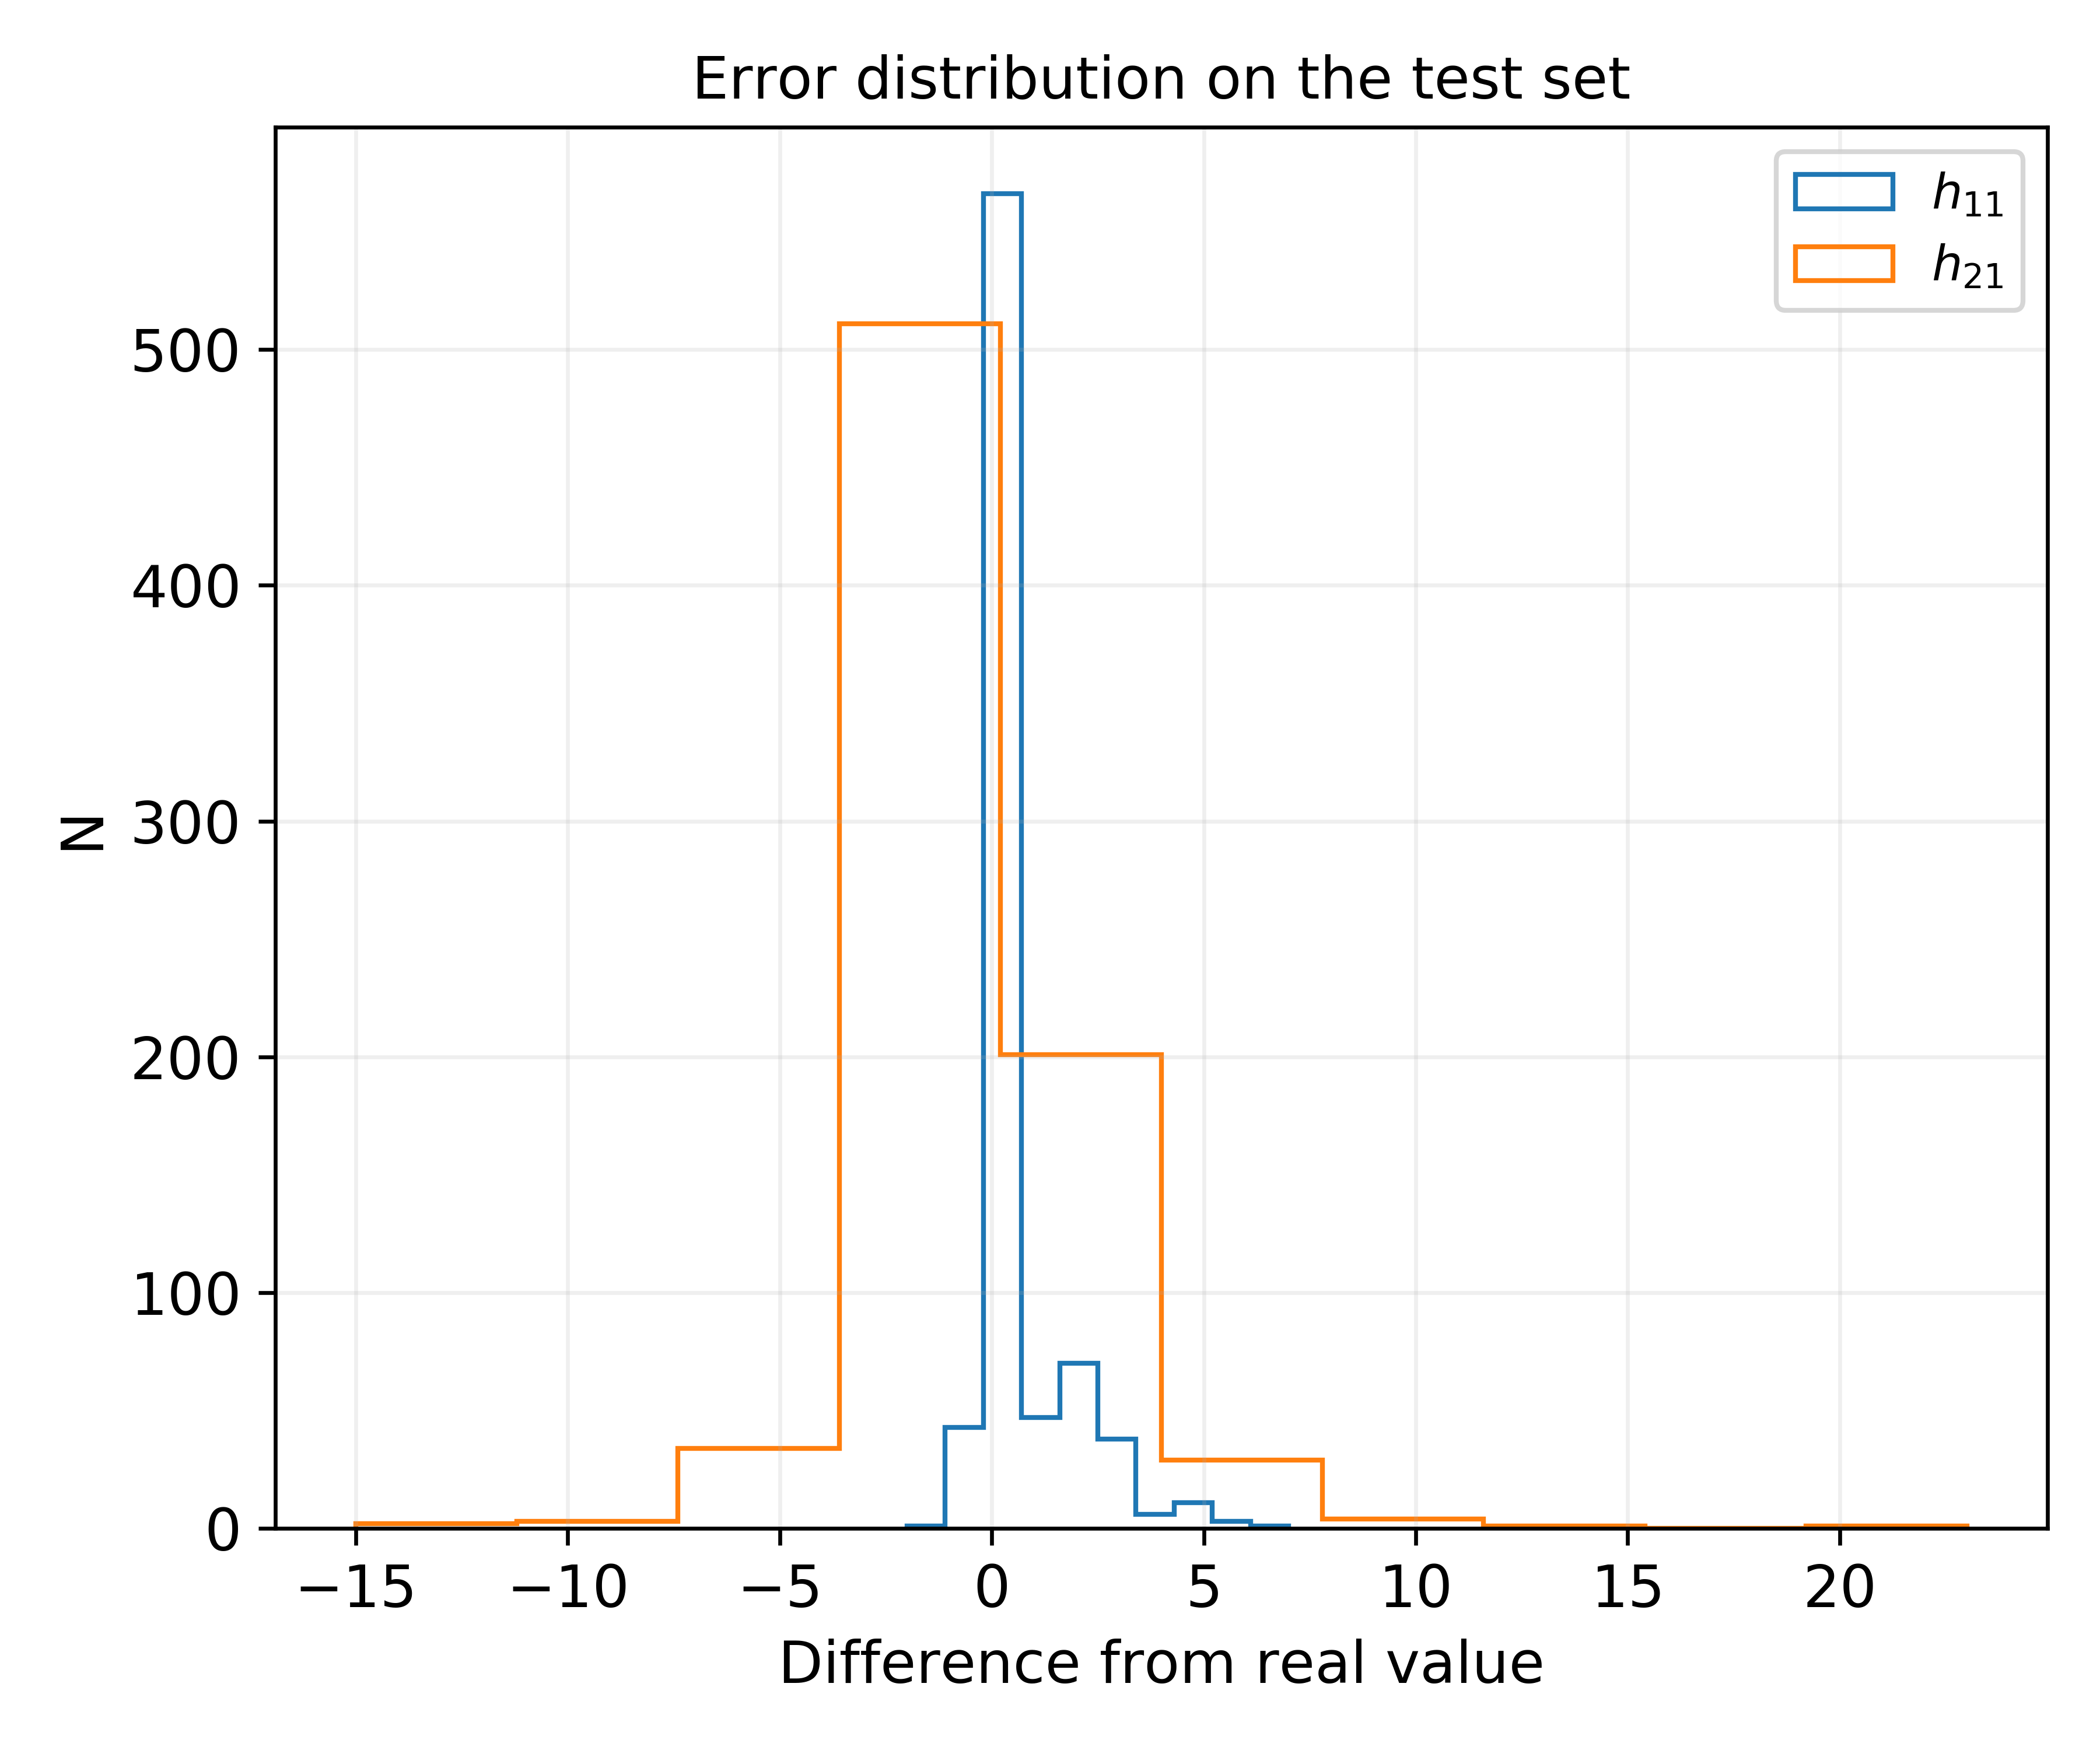
\includegraphics[width=0.75\textwidth]{tex/img/svr_rbf_error_eng.png}
        \caption{Error distribution for \texttt{SVR} with \textit{rbf} kernel using the engineered dataset.}
        \label{fig:svr_rbf_err}
    \end{figure}
    
\subsection{Random Forest}
    We eventually consider the \texttt{RandomForestRegressor}. We implement a search space for the \texttt{BayesSearchCV} for the hyperparameters \texttt{criterion}, \texttt{max\_depth}, \texttt{min\_samples\_leaf}, \texttt{min\_samples\_split} and \texttt{n\_estimators} and we use the \textit{floor} function for the accuracy.
    
    The naive computation with only the matrix components for $h_{11}$ reached $61.5\% \pm 1.4\%$ of accuracy during cross-validation and $61.7\%$ of accuracy for the test predictions using \texttt{criterion = friedman\_mse}, \texttt{max\_depth = $20$}, \texttt{min\_samples\_leaf = $1$}, \texttt{min\_samples\_split = $10$} and \texttt{n\_estimators = $64$}. The same computation for $h_{21}$ led to $14.8\% \pm 1.1\%$ during cross-validation and $14.8\%$ of accuracy in the test set using \texttt{criterion = mae}, \texttt{max\_depth = $20$}, \texttt{min\_samples\_leaf = $1$}, \texttt{min\_samples\_split = $2$} and \texttt{n\_estimators = $75$}.
    
    The baseline computation with \texttt{num\_cp} only for $h_{11}$ reached $62\% \pm 2\%$ of accuracy during cross-validation and $63\%$ of accuracy during the test predictions using \texttt{criterion = mae}, \texttt{max\_depth = $9$}, \texttt{min\_samples\_leaf = $1$}, \texttt{min\_samples\_split = $2$} and \texttt{n\_estimators = $5$} For $h_{21}$ we find $11.1\% \pm 1.1\%$ of accuracy in cross-validation and $10.4\%$ for the test set using \texttt{criterion = mae}, \texttt{max\_depth = $8$}, \texttt{min\_samples\_leaf = $4$}, \texttt{min\_samples\_split = $10$} and \texttt{n\_estimators = $6$}.
    
    The second baseline computation using only \texttt{dim\_cp} shows a small improvement for $h_{11}$ with $65\% \pm 2\%$ in cross-validation and $66\%$ of accuracy for the test predictions with \texttt{criterion = mae}, \texttt{max\_depth = $6$}, \texttt{min\_samples\_leaf = $1$}, \texttt{min\_samples\_split = $2$} and \texttt{n\_estimators = $42$}, while the results for $h_{21}$ are $13.9\% \pm 1.3\%$ of accuracy in cross-validation and $14.4\%$ for the test set using \texttt{criterion = mae}, \texttt{max\_depth = $7$}, \texttt{min\_samples\_leaf = $2$}, \texttt{min\_samples\_split = $3$} and \texttt{n\_estimators = $2$}.
    
    The complete computation using the engineered features does not show great improvement both for $h_{11}$ and $h_{21}$. Specifically we get $65.4\% \pm 1.4\%$ of accuracy in cross-validation for $h_{11}$ and $64.8\%$ during the test predictions using \texttt{criterion = mae}, \texttt{max\_depth = $10$}, \texttt{min\_samples\_leaf = $1$}, \texttt{min\_samples\_split = $10$} and \texttt{n\_estimators = $63$}, while the accuracy for $h_{21}$ is $21.1\% \pm 1.6\%$ of accuracy during cross-validation and $16.8\%$ during the test predictions using \texttt{criterion = friedman\_mse}, \texttt{max\_depth = $20$}, \texttt{min\_samples\_leaf = $1$}, \texttt{min\_samples\_split = $2$} and \texttt{n\_estimators = $75$}. We show in Figure~\ref{fig:rnd_for_err} the distribution of the the errors of the test predictions.
    
    \begin{figure}[t]
        \centering
        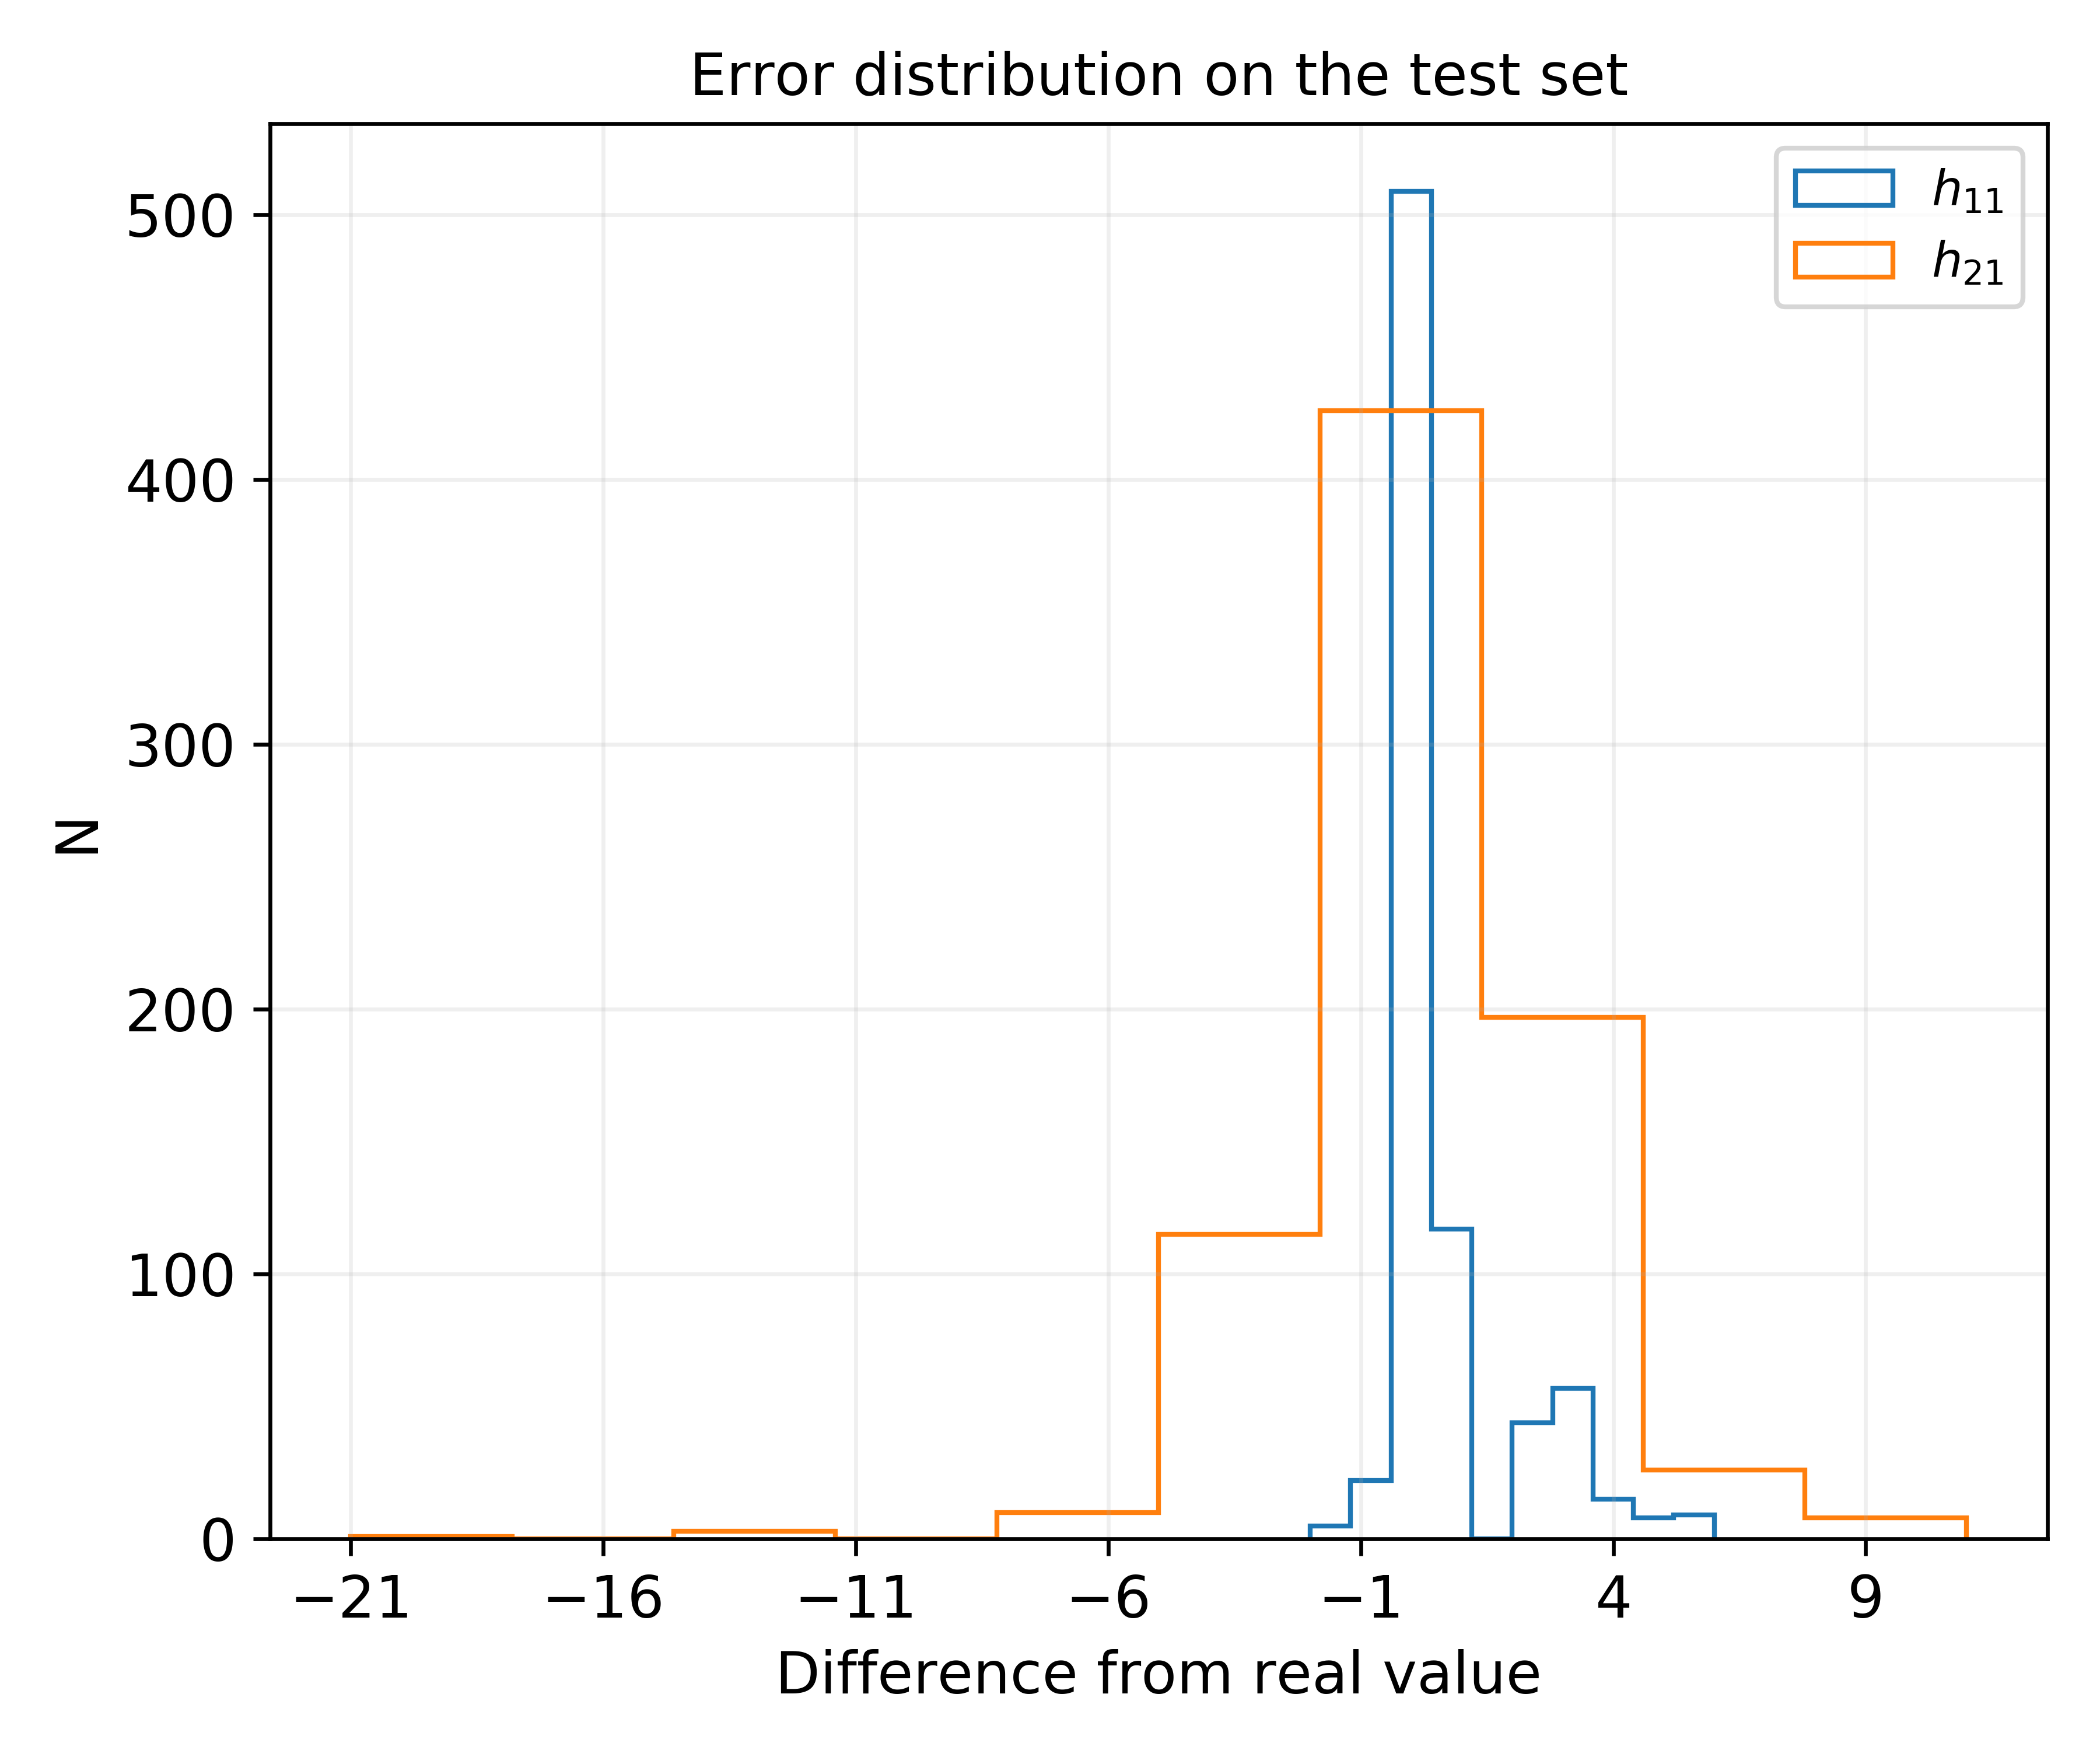
\includegraphics[width=0.75\textwidth]{tex/img/rnd_for_error_eng.png}
        \caption{Error distribution for \texttt{RandomForestRegressor} using the engineered dataset.}
        \label{fig:rnd_for_err}
    \end{figure}
    
\subsection{CNN (v1)}

    \subsubsection{Sequential Model}
        As a first approach to the problem, we use a CNN applied to the configuration matrix (mind that the it is a $12 \times 15$ matrix with $180$ entries) of the manifolds. The idea is to let the network decide which features should be used to predict the Hodge numbers using kernel transformations. We use two different architectures to predict $h_{11}$ and $h_{21}$ separately.
        
        We first consider the architecture to predict $h_{11}$. We use one input layer (\texttt{Conv2D} with \texttt{kernel\_size = $5$} and $80$ filters) and two hidden layers (\texttt{Conv2D} with \texttt{kernel\_size = $5$} and $40$ and $20$ filters, respectively). We then flatten the result thus getting a new input vector with $12 \times 15 \times 20 = 3600$ components. We then attach a simple deep neural network to manipulate the result: we use one \texttt{Dense} layer of $800$ neurons and one output layer with $1$ neuron. In all cases we also apply a $l1$ regularization of $10^{-5}$ to the kernel. We use \textit{ReLU} as activation function for each layer (also for the output layer since we are interested in positive predictions) and batch normalisation after each activation layer. We also insert a \texttt{Dropout} layer (\texttt{rate = $0.2$}) after the \texttt{Flatten} layer. In this case the size of each batch of data is $16$ with a learning rate of $0.001$.
        
        We then consider the architecture for $h_{21}$ which is inevitably more complicated. We use one input layer (\texttt{Conv2D} with \texttt{kernel\_size = 6} and $180$ filters) and five hidden layer (all \texttt{Conv2D} with \texttt{kernel\_size = $6$} and $150$, $150$, $100$, $50$ and $20$ filters, respectively). We then flatten the output to get another $3600$ components vector. We then apply a \texttt{Dropout} layer (\texttt{rate = 0.4}) and attach a \texttt{Dense} layer with $30$ neurons and one output layer with $1$ neuron. In this case we do not use $l1$ or $l2$ regularisation. We use \textit{ReLU} as activation function for each layer (including the output), followed by batch normalisation. In this case the batch size is $32$ with a learning rate of $0.001$.
        
        As the results will show, this is probably the best case scenario concerning the neural networks because we do not insert any manipulation of the input. In fact, through kernel transformations, we let the network decide which features are best to use. In fact, as we will see, manually adding features usually leads to worse results\footnote{One possible way to further explore this would be to build deeper networks with more layers and more filters. However my laptop has only 2 GB of GPU RAM which are quickly filled and Google's \textit{CoLab}, though valuable, is not stable enough for long training.}.
        
        With this setup we reach $90\%$ of accuracy on the validation set and the test set for $h_{11}$ after 230 epochs, while we reach $34\%$ of accuracy on the validation and test sets for $h_{21}$ after 163 epochs.
    
    \subsubsection{Functional Model}
        We then try to elaborate more the previous model by adding manually studied features such as \texttt{num\_cp}, \texttt{dim\_cp} and \texttt{dim\_h0\_amb}. Since the first is simply a scalar feature, we will use only \texttt{Dense} layers for \texttt{num\_cp} while the other vector features will first go through \texttt{Conv1D} layers to be manipulated.
        
        The architecture will therefore theoretically be as follow:
        \begin{itemize}
            \item build a DNN for \texttt{num\_cp},
            \item build a CNN for \texttt{dim\_cp} and \texttt{dim\_h0\_amb},
            \item use the previously built CNN for \texttt{matrix},
            \item concatenate the networks:
                \subitem \texttt{num\_cp}, \texttt{dim\_cp}, \texttt{matrix} for $h_{11}$,
                \subitem \texttt{num\_cp}, \texttt{dim\_cp}, \texttt{dim\_h0\_amb}, \texttt{matrix} for $h_{21}$,
            \item add a small DNN to \texttt{num\_cp}, \texttt{dim\_cp}, \texttt{matrix} to output $h_{11}$,
            \item reinforce the input by concatenating the output layer for $h_{11}$ with \texttt{dim\_cp} as in Residual Neural Networks (RNN) and process them through a very small DNN,
            \item concatenate this sub-network with \texttt{num\_cp}, \texttt{dim\_cp}, \texttt{dim\_h0\_amb}, \texttt{matrix} to output $h_{21}$ (attach a very small DNN to process all the information).
        \end{itemize}
        The final model will however be simpler due to the nature of the inputs.
        
        In this model we do not implement kernel regularisation as there are very different features that have been shown to react very differently under $l1$ or $l2$ regularisation. In fact adding such factors usually spoils the result and finding the correct balance is a very difficult fine tuning procedure which could take a huge amount of time. In the end we decided to avoid using it. We use \textit{ReLU} as activation function (including the output layers) and batch normalisation after it.
        
        Since \texttt{num\_cp} is linearly connected to $h_{11}$ and $h_{21}$ we do not insert hidden layers. The same goes for \texttt{dim\_cp} which gets immediately flattened and concatenated. \texttt{dim\_h0\_amb} goes through two hidden \texttt{Conv1D} layers with $20$ and $10$ filters each before being flattend into a $15 \times 10 = 150$ components vector. For the 1D convolutional layers we use a kernel size of $2$. After the first concatenations we add a \texttt{Dropout} layer (\texttt{rate = 0.2} for $h_{11}$ and \texttt{rate = 0.4} for $h_{21}$). We then attach a small DNN to the output of $h_{11}$ concatenated with a residual connection to \texttt{dim\_cp} (two hidden \texttt{Dense} layers with $20$ and $10$ neurons each). We then concatenate this with \texttt{num\_cp}, \texttt{dim\_cp}, \texttt{dim\_h0\_amb} and \texttt{matrix} and a hidden layer with $10$ neurons before attaching everything to the output layer for $h_{21}$.
        
        With this architecture we reach $84\%$ of accuracy both on the validation set and the test set for $h_{11}$ and $32\%$ on both sets for $h_{21}$.
        
    \subsubsection{Other Models}
        As a training exercise, we also implemented two more different neural network architectures: one using the \texttt{PCA} results instead of the matrix and treating it through a \textit{ConvNet} and one using the \texttt{PCA} results through a FC network. Their results are irreparably worse with respect to the previous architectures (below $70\%$ of accuracy for $h_{11}$ and below $20\%$ for $h_{21}$) and will not be considered for the stacking ensemble.
        
\subsection{Stacking Ensemble}
    Eventually we also present the results we got using an ensemble approach through stacking. Using the analysis discussed in Section~\ref{sec:ensemble_desc}, even though the algorithms perform in general a bit worse with respect to the previous analysis due to the smaller training set, we reach $91\%$ of accuracy on $h_{11}$ using \texttt{SVR} (Gaussian kernel) as meta learner and \texttt{RobustScaler} applied to the second level set, thus showing an improvement of $2\%$ with respect to the sequential model which proved to be the best result on the training set in this analysis. We also get $38\%$ of accuracy on $h_{21}$ using \texttt{RandomForestRegressor} as meta learner and no scalers applied to the second level set: we improve the result of the best model in the stacking analysis, the functional CNN\footnote{Notice that when using the ``full'' training set (i.e. $80\%$ of the total dataset) the functional CNN does not perform as well the sequential CNN, but when using less entries of the dataset (i.e. only $50\%$ of the entire dataset) the functional CNN matches the accuracy of the CNN on the full training set for $h_{11}$ and it outperforms it for $h_{21}$.}, by $4\%$.
    
    Notice that with the stacking ensemble we also improved the results given by the analysis of the previous sections: specifically we improve the accuracy on $h_{11}$ by $1\%$ and by $4\%$ on $h_{21}$ with respect to the sequential CNN which held the best results.